% ============================================================================================================
\chapter{Analyse de sensibilité}\label{ch:sensibilite}
% ============================================================================================================

\section{Le paramètre de transmission vers le potentiel}

Le paramètre qui faisait varier la dette de S3 en 2047 de $-9$ à $+43$ points en v0.7 est traité au
chapitre~\ref{ch:equations} : il est remplacé par deux paramètres estimés (ρ, rappel de la production vers le
potentiel ; θ, part de la variation du potentiel anticipée par la demande) dont les valeurs sont contraintes par la
durée empirique des écarts de production (AMECO et FMI, 1982-2019) et par la réaction de la consommation aux chocs
permanents de revenu. Les conclusions de cette estimation :
\begin{itemize}
\item \textbf{pas d'estimation ponctuelle robuste} : l'ensemble des couples (ρ, θ) compatibles avec la durée empirique
(1,6 à 5,3 ans) est large ; on retient une plage, θ entre 0,5 et 1,0 et ρ entre 0,1 et 0,3, et une valeur centrale
(θ = 0,75 ; ρ = 0,2) au milieu de cette plage, \emph{choisie avant} de regarder les résultats des stratégies ;
\item \textbf{pas d'asymétrie ni de dépendance à l'état détectables} (statistiques $t$ de 0,03 à 1,5) : une
spécification à paramètres constants est retenue, faute de mieux ; les données (une quarantaine d'années, quelques
cycles) ne permettent pas d'estimer des paramètres sectoriels ou par type de choc ;
\item \textbf{le backtest ne départage pas} les valeurs de θ (chapitre~\ref{ch:backtest}) : la période 2010-2019 contient
peu de chocs d'offre identifiables.
\end{itemize}

\section{Sensibilité un à un}

Chaque paramètre est placé à sa valeur basse puis haute, les autres à leur valeur centrale, et la référence est
recalculée avec les mêmes paramètres. Pour limiter le temps de calcul (douze paramètres, deux valeurs, cinq
stratégies : 120 simulations), le module de la zone euro est désactivé ; les valeurs centrales diffèrent donc de celles
du chapitre~\ref{ch:strategies} (voir l'encadré), et seules les \emph{amplitudes} sont à lire ici.

\begin{figure}[htbp]\centering
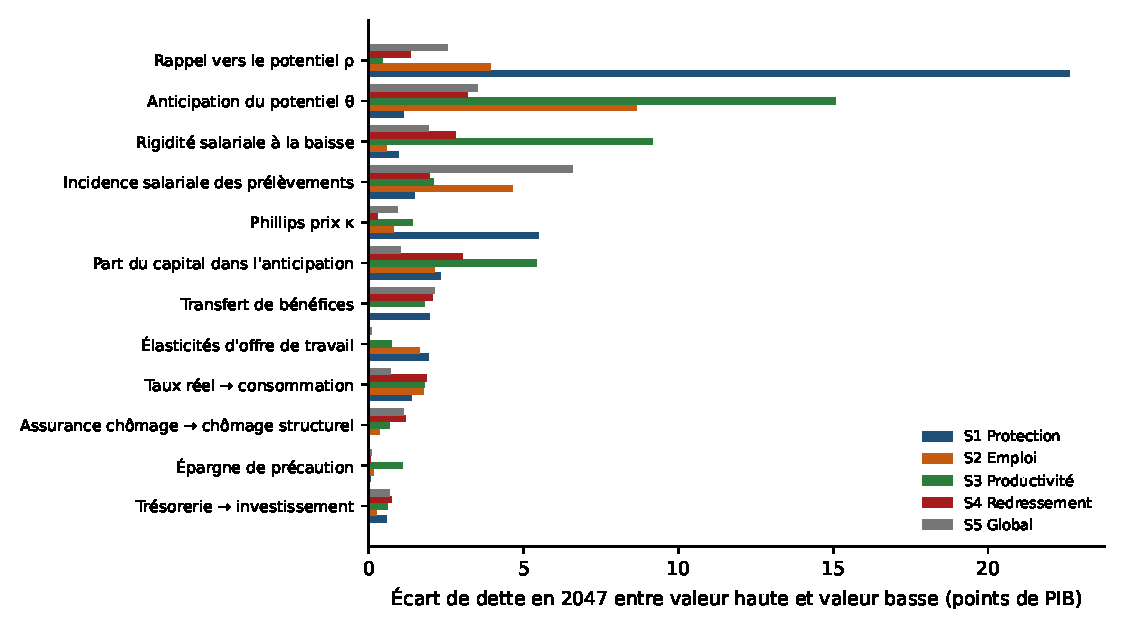
\includegraphics[width=\linewidth]{sensibilite.pdf}
\caption{Amplitude de l'effet de chaque paramètre sur la dette publique en 2047 (écart entre valeur haute et valeur
basse), par stratégie.}\label{fig:sens}
\end{figure}

\begin{table}[htbp]\centering\scriptsize
\caption{Dette publique en 2047 (écart à la référence, points de PIB) : valeur centrale et [valeur basse ; valeur haute]
de chaque paramètre ; paramètres classés par amplitude maximale.}\label{tab:sens_dette}
\tabfit{../tables/sensibilite_dette.tex}
\end{table}

\begin{table}[htbp]\centering\scriptsize
\caption{PIB en volume en 2047 (écart à la référence, \%).}\label{tab:sens_pib}
\tabfit{../tables/sensibilite_pib.tex}
\end{table}

\paragraph{Classement.} Trois paramètres dominent :
\begin{itemize}
\item \textbf{ρ, le rappel vers le potentiel}, pour S1 : de $-10$ à $+13$ points de dette en 2047. S1 est une stratégie
de demande ; plus la production revient vite vers son potentiel, plus l'effet d'activité qui finance une partie des
mesures s'éteint vite ;
\item \textbf{θ, l'anticipation du potentiel}, pour les stratégies d'offre : S3 de $+27$ à $+42$ points, S2 de $+10$ à
$+19$. Plus la demande anticipe la hausse du potentiel, plus la production rejoint vite le potentiel accru, et plus les
recettes suivent ;
\item \textbf{la rigidité salariale à la baisse} pour S3 ($+31$ à $+40$) et \textbf{l'incidence salariale des
prélèvements} pour S5 ($-2$ à $+4$ : le signe de l'effet de S5 sur la dette en dépend).
\end{itemize}
Les paramètres de comportement des entreprises (trésorerie, transfert de bénéfices) et de consommation (précaution,
taux réel) déplacent la dette de 2047 de moins de 3 points. Les élasticités d'offre de travail comptent pour le PIB de
S1 et de S3 (0,2 à 0,3 point), peu pour la dette.

\begin{resultat}[Ce qui est robuste aux paramètres]
Le signe et l'ordre des effets sur la dette en 2047 ne changent pas pour S2, S3 et S4 sous aucune des 24 variations : S4
réduit fortement la dette (de 41 à 46 points), S3 l'augmente (27 à 42), S2 l'augmente (10 à 19). Pour S1 et S5, l'effet
est proche de zéro et son signe dépend de ρ (S1) ou de l'incidence (S5). Le PIB de 2047 est plus robuste : l'ordre
S3 > S2 > S5 > S1 > S4 n'est jamais modifié.
\end{resultat}

\begin{encadre}{Une source d'incertitude structurelle sous-estimée en v0.7 : la zone euro}
Avec le module de la zone euro (réaction de la BCE à l'inflation et à l'activité de la zone, commerce avec les
partenaires), les effets sur la dette sont nettement plus marqués : S4 $-59$ points en 2047 au lieu de $-43$, S3 $+53$
au lieu de $+34$, S2 $+26$ au lieu de $+15$. \par\medskip{\centering\scriptsize\begin{tabular}{lrrrrrrr}\toprule
 & \multicolumn{4}{c}{Dette 2047 (points)} & \multicolumn{3}{c}{Intérêts 2047 (points de PIB)} \\\cmidrule(lr){2-5}\cmidrule(lr){6-8}
 & sans M11 & prime 0 & 0,03 & 0,05 & prime 0 & 0,03 & 0,05 \\ \midrule
S1 Protection & $+4$ & $+8$ & $+10$ & $+11$ & $+0{,}6$ & $+1{,}0$ & $+1{,}3$ \\
S2 Emploi & $+15$ & $+18$ & $+26$ & $+33$ & $+1{,}2$ & $+2{,}7$ & $+4{,}3$ \\
S3 Productivité & $+34$ & $+37$ & $+53$ & $+69$ & $+2{,}0$ & $+5{,}4$ & $+9{,}0$ \\
S4 Redressement & $-43$ & $-44$ & $-59$ & $-72$ & $-2{,}0$ & $-4{,}9$ & $-7{,}4$ \\
S5 Global & $+2$ & $+3$ & $+5$ & $+7$ & $+0{,}3$ & $+0{,}7$ & $+1{,}1$ \\
\bottomrule\end{tabular}\par}\medskip
 La réaction de la BCE et le commerce avec la zone euro comptent peu (colonne « prime 0 ») : 1 à 4 points de dette. L'essentiel vient de la \emph{prime de risque} sur les taux français, de 0,03 point de taux long par point de dette (hypothèse de niveau C, au milieu des estimations de la littérature, 0,02 à 0,05) : un écart de dette se renchérit ou s'allège par les intérêts, et l'effet se cumule sur vingt ans. Pour S3, la dette de 2047 passe de $+$37 points sans prime à $+$53 avec la prime centrale et $+$69 avec une prime de 0,05. Cette hypothèse n'était pas variée dans les configurations faible et forte ; elle est désormais traitée comme une incertitude structurelle à part entière.

\end{encadre}
